\documentclass[tikz,border=2pt]{standalone}
\usepackage{amsmath,amssymb}
\usepackage{pgfplots}
\pgfplotsset{compat=1.18}

\begin{document}
% Joint density 2 on the triangle 0 < x < y < 1 and zero elsewhere. The probability of a region
% is the integral of the density over it: P(Y < 1/2) = 2 * (area 1/8) = 1/4.
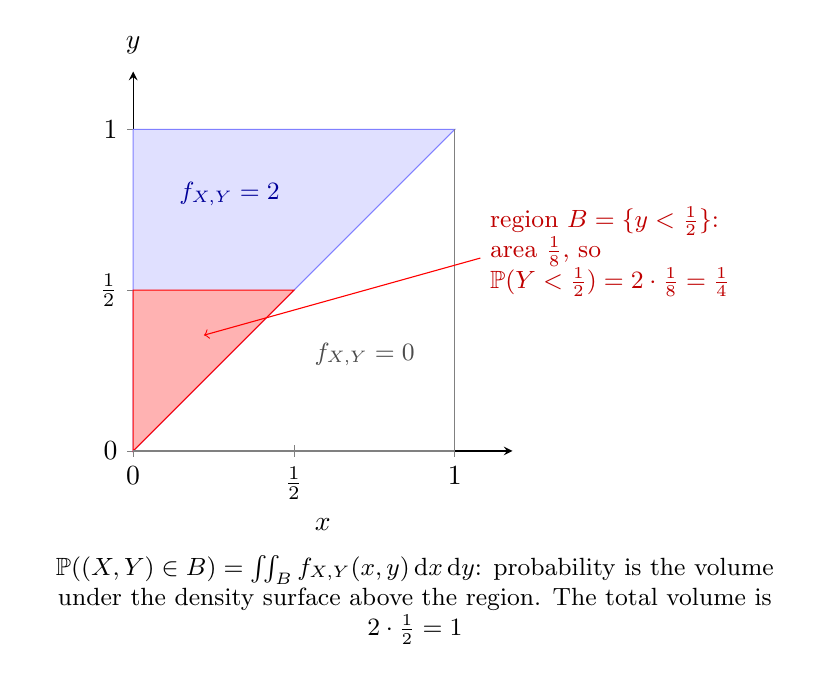
\begin{tikzpicture}
	\begin{axis}[
		axis lines=left, xmin=0, xmax=1.18, ymin=0, ymax=1.18,
		xtick={0,0.5,1}, xticklabels={$0$,$\tfrac12$,$1$}, ytick={0,0.5,1}, yticklabels={$0$,$\tfrac12$,$1$},
		xlabel={$x$}, ylabel={$y$}, ylabel style={rotate=-90, anchor=south, at={(axis description cs:0,1.02)}},
		width=6.4cm, height=6.4cm, clip=false
		]
		\addplot[fill=blue!12, draw=blue!50] coordinates {(0,0) (1,1) (0,1)} -- cycle;
		\addplot[fill=red!30, draw=red] coordinates {(0,0) (0.5,0.5) (0,0.5)} -- cycle;
		\draw[gray] (axis cs:0,0) -- (axis cs:1,0) -- (axis cs:1,1);
		\node[blue!60!black, font=\small] at (axis cs:0.3,0.8) {$f_{X,Y}=2$};
		\node[gray!60!black, font=\small] at (axis cs:0.72,0.3) {$f_{X,Y}=0$};
		\node[red!75!black, anchor=west, font=\small, align=left] at (axis cs:1.08,0.62) {region $B=\{y<\tfrac12\}$:\\ area $\tfrac18$, so\\ $\mathbb{P}(Y<\tfrac12)=2\cdot\tfrac18=\tfrac14$};
		\draw[red, ->] (axis cs:1.08,0.6) -- (axis cs:0.22,0.36);
	\end{axis}
	\node[anchor=north, font=\small, align=flush center, text width=9.6cm] at ([yshift=-2pt]current axis.outer south) {$\mathbb{P}((X,Y)\in B)=\iint_Bf_{X,Y}(x,y)\,\mathrm{d}x\,\mathrm{d}y$: probability is the volume under the density surface above the region. The total volume is $2\cdot\tfrac12=1$};
\end{tikzpicture}
\end{document}
